\chapter{Unpublished Work and Open Mysteries}
\label{ch:unpublished}

Many promising projects have been abandoned over the course of my thesis work due to limited brain bandwidth, and due to the previous five chapters showing more promising and clear results.
In the following sections, I will briefly outline progress that has been made on some of these abandoned projects, in the hope that they can be revisited and completed in the future.

\section{Flywheel Modes in 2D Convection}
\label{sec:flywheels}
This project \emph{almost} became a paper, but we couldn't find an angle in which to make it sufficiently interesting.
Our goal was to study \RB convection at \textbf{high aspect ratio with stress free boundaries}, and show:
\begin{enumerate}
\item An argument for how the average system enstrophy should scale as a function of Ra (see section \ref{sec:enstrophy_scaling}).
\item A description of the physical mechanism that creates this enstrophy (see section \ref{sec:enstrophy_generation}).
\item A description of the timescales over which flywheels spin up (or down, depending on thermal boundary condition choice).
Presumably this is related to the viscous diffusion timescale, but it's a bit unclear what it is.
\item A comparison to no-slip sims, and whether they have a similar spin-up (how do they avoid these modes?).
\item A demonstration of what you get wrong if you take your measurements before the spin-up is done at high Ra (I think you probably get flux-related quantities like Nu right but velocity-related quantities like Re wrong).
\end{enumerate}

\subsection{An argument for the scaling of enstrophy in a Boussinesq, convective system}
\label{sec:enstrophy_scaling}
The Boussinesq momentum equation, nondimensionalized on a freefall timescale, is
\begin{equation}
\pderiv{\bu}{t} = -\grad\varpi + T_1\hat{z} - \mR \dotp{\bu}{\curl{\bV}} + \cross{\bu}{\bV},
\label{eqn:momentum}
\end{equation}
where $\bu$ is the velocity vector, $\varpi$ is the reduced pressure (a Lagrange multiplier that enforces incompressibility), $T_1$ is the temperature deviation from background, $\mR = \sqrt{\text{Pr}/\text{Ra}}$, and $\bV = \curl{\bu}$ is the vorticity.
We dot $\bu$ into this equation in order to get the kinetic energy equation,
\begin{equation}
\pderiv{u^2/2}{t} + \Div{\varpi \bm{u} + \mR \cross{\bV}{\bu}} = w T_1 - \mR \omega^2.
\end{equation}
Under the assumption of impenetrable boundaries ($w = 0$, so $w\varpi = 0$), coupled with no-slip ($\bu = 0$) or stress-free boundaries ($\bV = 0$), the fluxes disappear at the top and bottom plate.
So -- kinetic energy cannot exit the domain through the boundaries, but must instead be generated and destroyed by the source and sink terms.
If we define the volume average as $\angles{} = \mathcal{V}^{-1}\int_{\mathcal{V}} dV$, where $\mathcal{V}$ is the volume of our domain, and we take the volume average of this equation, we get
\begin{equation}
\angles{\pderiv{u^2/2}{t}} = \angles{w T_1} - \mR \angles{\omega^2}.
\end{equation}
Assuming that the kinetic energy in the convection reaches a steady state, the LHS of this expression disappears and we find,
\begin{equation}
\angles{\omega^2} = \mR^{-1} \angles{w T_1},
\end{equation}
the evolved value of the \emph{enstrophy}, $\omega^2$, is determined by the evolved value of the convective heat transport.
The heat transport can be expressed in terms of the Nusselt number, 
\begin{equation}
\text{Nu} \equiv 1 + \frac{\angles{w T_1}}{-\mP \angles{\partial_z (T_0 + T_1)}},
\end{equation}
where $\mP = \mR/\text{Pr}$, and in an equilibrated state
\begin{equation}
\angles{w T_1} = 
\begin{cases}
\mP (\text{Nu} - 1)  & \text{TT boundaries}, \\
\mP (1 - \text{Nu}^{-1}) & \text{FT or FF boundaries}
\end{cases}.
\end{equation}
Or, through a straightforward substitution, we expect
\begin{equation}
\angles{\omega^2} = 
\begin{cases}
\text{Pr}^{-1} (\text{Nu} - 1)  & \text{TT boundaries}, \\
\text{Pr}^{-1} (1 - \text{Nu}^{-1}) & \text{TT or FT boundaries}
\end{cases}.
\end{equation}
We find that this is indeed a good description of the enstrophy contained in the evolved flywheels for stress-free simulations, see Fig. \ref{fig:enstrophy}.
Note, these scalings hold up for no-slip boundary conditions, as well.
In the case of no-slip boundaries, the enstrophy is localized near the boundary (where the bulk velocities must go to zero over a small length scale of the boundary layer thickness).

\begin{figure}[t!]
    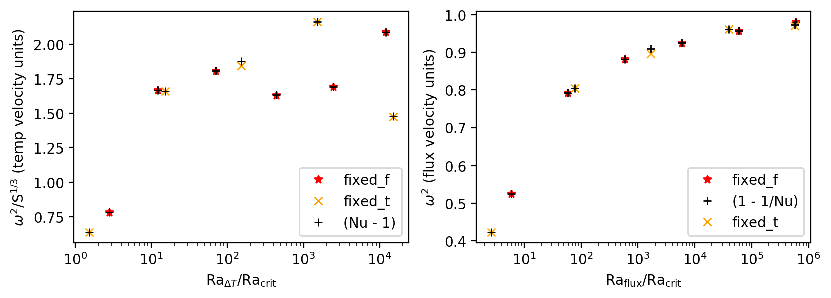
\includegraphics[width=\textwidth]{figs/unpublished/enstrophy_v_ra.pdf}
    \caption[Evolved enstrophy in RBC simulations.]{
	(left) Enstrophy in inverse freefall time units nondimensionalized by the evolved temperature jump across the domain, and normalized by the supercriticality to the third power.
	(right) Enstrophy in inverse freefall time units nondimensionalized by the evolved system flux.
	Simulation measurements are shown from simulations run with FF boundaries (red stars), TT boundaries (orange crosses), and the expected value of enstrophy as a function of Nu is overplotted.
    \label{fig:enstrophy} }
\end{figure}

\subsection{Where does the enstrophy come from?}
\label{sec:enstrophy_generation}
In order to determine where the enstrophy comes from, we first curl Eqn.~\ref{eqn:momentum} to retrieve the vorticity equation,
\begin{equation}
\pderiv{\bV}{t} = -(\dotp{\bu}{\grad})\bV + (\dotp{\bV}{\grad})\bu + \curl{T_1\hat{z}} + \mR \grad^2 \bV.
\end{equation}
We now dot $\bV$ into this equation to retrieve the enstrophy evolution equation,
\begin{equation}
\pderiv{\omega^2/2}{t} + \Div{\cross{\bV}{\left(T_1\hat{z} - \mR\curl{\bV} + \cross{\bu}{\bV}\right)}} = \dotp{\left(T_1\hat{z} - \mR\curl{\bV} + \cross{\bu}{\bV}\right)}{\curl{\bV}}.
\end{equation}
We are specifically interested in the 2D case where $\bu = u\hat{x} + w\hat{z}$ and $\bV = \omega\hat{y}$.
In this limit, the enstrophy equation is
\begin{equation}
\begin{split}
\pderiv{\omega^2/2}{t} + \Div{\omega\left[\left(T_1 + u\omega - \mR\pderiv{\omega}{x}\right)\hat{x} + \left(w\omega - \mR\pderiv{\omega}{z}\right)\hat{z}\right]} 
=\\ T_1\pderiv{\omega}{x} + \frac{1}{2}\left(w\pderiv{\omega^2}{z} + u\pderiv{\omega^2}{x}\right) - \mR \left(\left[\pderiv{\omega}{z}\right]^2 + \left[\pderiv{\omega}{x}\right]^2\right).
\end{split}
\end{equation}
We can see immediately that all enstrophy fluxes vanish at the boundaries for stress-free boundary conditions (where $\bV = 0$ at the boundaries).
For this case, we take a volume average and find:
\begin{equation}
\angles{\pderiv{\omega^2}{t}} = 2\angles{T_1\pderiv{\omega}{x}} + \angles{w\pderiv{\omega^2}{z} + u\pderiv{\omega^2}{x}} - 2\mR \angles{\left[\pderiv{\omega}{z}\right]^2 + \left[\pderiv{\omega}{x}\right]^2}.
\end{equation}
On the RHS, there are three source terms for the enstrophy.
From left to right, they are the baroclinic term (from buoyancy), a term from advection (vortex stretching), and viscous dissipation.
Viscosity acts in a straightforward way: it aims to reduce enstrophy anywhere there is a gradient of the vorticity.
Buoyancy also acts in a fairly straightforward way: Downflows ($T_1 < 0$) separate areas of positive vorticity (on the left) and negative vorticity (on the right), meaning $\pderiv{\omega}{x} < 0$, and produce a net positive enstrophy.
Upflows act in the same way, where the signs on both terms are switched and the product remains positive.
The advective term is more complicated.
The $u \pderiv{\omega^2}{x}$ term seems to destroy enstrophy at plume generation sites and produce it at plume impacting sites.
The $w \pderiv{\omega^2}{z}$ term seems to both generate and destroy enstrophy at  impacting sites (probably canceling out), but it generates enstrophy at plume launching sites.

Initial simulation results suggest that the advective generation terms are unimportant, and average out to about zero across the domain.
It seems that the baroclinic term generates enstrophy and the viscous term destroys it.
When these two terms come into balance, the flywheel is fully developed.

\subsection{Next steps}
Unfortunately, this was as far as this work progressed.
Logical next steps would be to figure out the timescales over which the flywheels develop (from theoretical efforts such as those laid out above, and from simulations).
Furthermore, carrying out a similar procedure for the compressible equations to understand if the flywheels are as simple to understand there would be crucial in understanding why our Mach number increases with Ra in 2D polytropic convection sims (in Fig.~\ref{fig:ma_v_eps}).
Finally, it would be fascinating to understand how the fully compressible equations dissipate flywheel energy at high Mach number (as in the high-Mach 2D cases in Fig.~\ref{fig:ma_v_eps}).

\section{The Magnitude of Viscous Terms in Turbulent Convection}
Historically, the magnitude of viscous terms (like viscous fluxes, and viscous heating) have been thought to be negligible in turbulent convection when diffusivities are small.
However, recent work by \citet{currie&all2017} has shown that the volume-integrated contributions of the viscous heating (viscous dissipation) term can exceed the luminosity of the convection, even at very high Rayleigh number.
Some of our unpublished work also suggests that viscous dissipation processes can be generally important in stratified convection.
For example, the shearing states that we discovered at low Mach number in Ch.~\ref{ch:ab17} had important contributions from the viscous flux.
In Fig.~\ref{fig:shear_fig}, a simulation with Ra = $10^{5.5}$ and $\epsilon = 10^{-4}$ (and otherwise constructed as described in Ch.~\ref{ch:ab17}) which displays shearing states is shown, including the large contributions from the viscous fluxes in those states.
An extension of the flywheel work, mentioned in the previous section, into the realm of stratified convection would likely be one of the best routes for understanding the importance and magnitude of viscous dissipation and viscous fluxes.

\begin{figure*}[p!]
    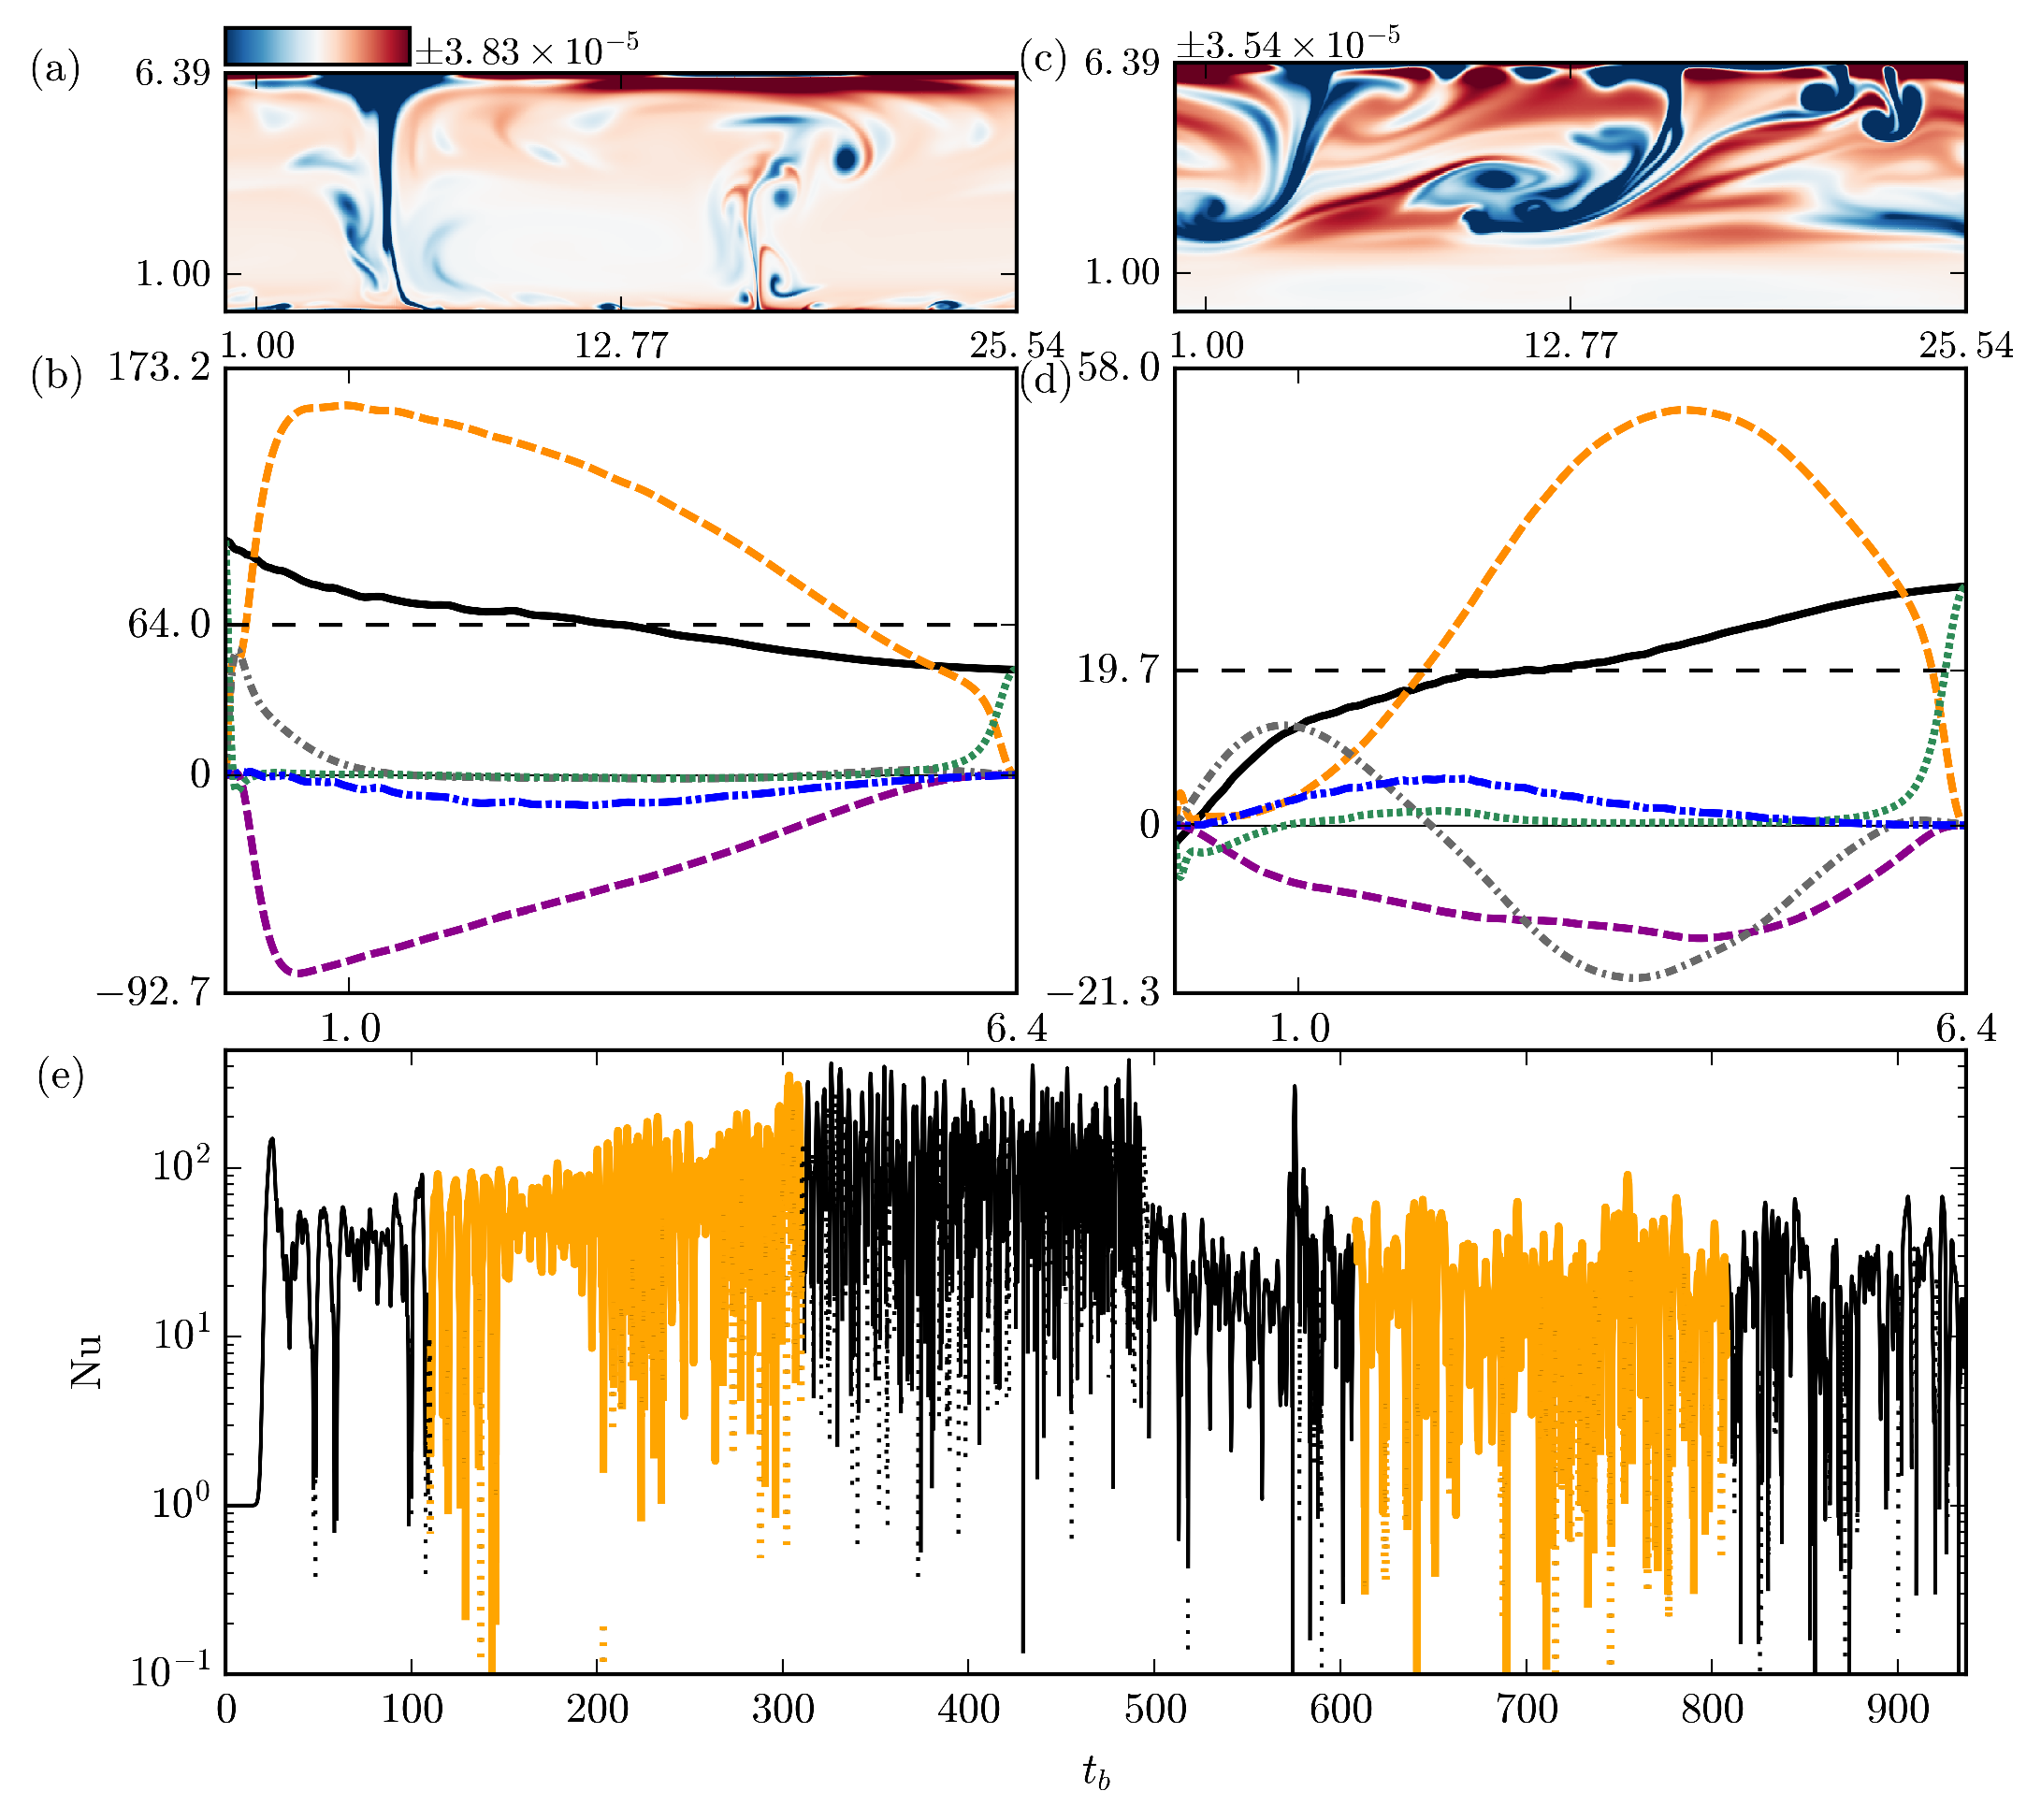
\includegraphics[width=\textwidth]{figs/unpublished/shear_fig.pdf}
    \caption[Shearing convection states in low Mach number, stratified convection.]{
	(a \& c) Entropy anomaly snapshots in low-Mach number, fully compressible convection in a classic roll (a) and shearing (c) state.
	(b \& d) The respective nondimensional fluxes in those systems.
	The dark black line shows the sum of the fluxes, and the yellow and purple dashed lines respectively show the enthalpy and kinetic energy fluxes.
	The conductive flux is shown as a dashed green line, and the potential energy flux is shown as a dash-dot-dot blue line.
	Interestingly, the viscous flux (dash-dot grey line) is never negligible.
	In the roll state, it is predominantly responsible for carrying the flux near the lower (stress-free) boundary.
	In the shearing state, it carries most of the flux in the lower part of the domain (and works against flux transport in the upper part of the domain.
	(e) A trace of the Nusselt number over time.
	The orange highlighted regions show the time windows over which averages were taken for the fluxes in the roll (left) and shearing (right) states, respectively.
	The overall magnitude of the flux in the shearing state, and thus the magnitude of Nu, is also very different.
    \label{fig:shear_fig} }
\end{figure*}





\section{Internally Heated, Fully Compressible Convection}
\label{sec:internally_heated}
Convective systems in nature (e.g., in stars) are generally not as simple as the purely boundary-driven convection generally examined in simulations.
The next step up in complexity from boundary driven convection is \emph{internally heated} convection, in which the convection is driven by deposition of energy in the bulk of the convective domain.
Two instances of internally heated convection in nature are the Sun and the Earth's mantle.
In the Sun, the increasing opacity within the solar convection zone (and subsequent divergence of radiative flux) leads to the gradual deposition of energy, as does radioactive decay in the Earth's mantle.
Understanding internally heated convection is therefore crucial for characterizing geophysical and astrophysical processes.
Inspired by the work of \citet{goluskin&spiegel2012} and the concise review of \citet{goluskin2016}, I had hoped to develop and study very simple internally heated, fully compressible systems.
Just as polytropic atmospheres have linear temperature profiles and can be compared to \RB convection easily, our goal was to develop and study stratified atmospheres driven by a constant (or linear) internal heating term, which would in turn produce quadratic (or cubic) temperature profiles which could be compared to internally heated Boussinesq convection.

\subsection{Preliminaries: convective stability and available flux}
\label{sec:stability}
In Boussinesq convection, convective stability is entirely determined by the temperature gradient.
There, negative temperature gradients drive convective motions, and positive temperature gradients are stable.
When compressibility is taken into account, atmospheres can maintain stability even in the presence of a large, negative temperature gradient \citep{spiegel&veronis1960}.
In such atmospheres, it is the gradient of \emph{entropy} which determines stability.
In an ideal gas, the specific entropy gradient is defined
\begin{equation}
\grad S = c_V \grad\ln T - R \grad\ln\rho,
\end{equation}
where $S$, $T$, and $\rho$ are the specific entropy, temperature, and density; $c_V$ is the specific heat at constant volume; and $R$ is the specific gas constant defining pressure, $P = R \rho T$.
Where stability is concerned, the entropy gradient in compressible systems is a direct analog to the temperature gradient in Boussinesq systems.
Regions with $\grad S < 0$ are unstable to convection, and regions with $\grad S > 0$ are stable.

Assuming that the convective system remains, to first order, in hydrostatic equilibrium, $\grad P = \rho \bm{g}$, the temperature gradient which characterizes a perfectly adiabatic state is:
\begin{equation}
\grad_{\text{ad}} = \bm{g}/c_P,
\end{equation}
where $\bm{g}$ is the gravity and $c_P$ is the specific heat at constant pressure.
The ``adiabatic temperature gradient,'' $\grad_{\text{ad}}$, can in general have a large magnitude, which makes the interpretation of the conductive (or radiative) flux in a system a bit harder to understand.
The conductive flux is
\begin{equation}
\bm{F}_{\text{cond}} = -\kappa \grad T,
\end{equation}
where $\kappa$ is the conductivity.
If a system is driven by some quantity of flux, $\bm{F}_{\text{drive}}$, we define the ``available flux'' as
\begin{equation}
\bm{F}_{\text{avail}} \equiv \bm{F}_{\text{drive}} - \bm{F}_{\text{ad}},
\end{equation}
where the ``adiabatic flux,'' $\bm{F}_{\text{ad}} = -\kappa\grad_{\text{ad}}$, is flux that can be conducted across an adiabatically stratified atmosphere.
If $\bm{F}_{\text{avail}} \leq 0$, the system is stable to convection.
If $\bm{F}_{\text{avail}} > 0$, the system is unstable to convection.
Importantly, $\bm{F}_{\text{avail}}$ is the \emph{only portion} of the flux that the convection is able to ``tap'' into.
Any amount of $\bm{F}_{\text{drive}}$ that is conducted down the adiabatic gradient will not be carried by convection.
Thus, $\bm{F}_{\text{avail}}$ is a direct analog in compressible systems to the \emph{total} flux carried through a Boussinesq system.

Internally heated (or cooled) convection in which the domain has a convecting region and a stable region is characterized by a heating (or cooling) profile that changes the sign of $\bm{F}_{\text{avail}}$.

\subsection{Disappearance of internal heating term from perturbation equations}
Given a constant internal heating term, $Q$ (in units of energy flux / length), the energy equation takes the form
\begin{equation}
\frac{D T}{Dt} + T(\gamma-1)\DivU = \frac{1}{\rho c_V}\left(\Div{\kappa \grad T} + Q\right) + \text{(Viscous Heating)}.
\end{equation}
In a static, steady state, thermal equilibrium in the ``background'' atmosphere satisfies 
\begin{equation}
-\Div{\kappa \grad T_0} = Q.
\end{equation}
Assuming that this thermal equilibrium is always met by the background profile (and for simplicity, assuming constant and uniform $\kappa$), the energy equation is
\begin{equation}
\frac{D T}{Dt} + T(\gamma-1)\DivU = \frac{1}{\rho c_V}\Div{\kappa \grad T_1} + \text{(Viscous Heating)}.
\label{eqn:energy_noheat}
\end{equation}

In other words, the equation for the perturbations is precisely the same as it is for a case where internal heating is not present, and the internal heating disappears from the system\footnote{
Note that this is \emph{precisely} true for simple, time-independent heating terms, $Q$, like the one we have discussed here.
However, astrophysical systems often have heating profiles which vary nonlinearly in time (which are either explicit heating terms, from sources like nuclear fusion, or pseudo-heating terms, from divergences of changing opacities as in Sec.~\ref{sec:kramers_opacity}).
The time-dependent portions of these heating terms would remain in Eqn.~\ref{eqn:energy_noheat}, even if a large O(1) portion of the heating term does not appear in the equation due to its cancellation with a background thermodynamic stratification.
}.
Internal heating therefore only enters the dynamics by modifying the background profile $T_0$ from a linear profile to something more complex.
The differences in this temperature profile affect dynamics through, for example, the $\bm{u}\cdot\grad T_0$ term in the temperature equation.
But -- importantly -- \emph{dynamics do not directly feel the source term}.

%%%%%%%%%%%%
%%%%%%%%%%%
% Atmospheres
%%%%%%%%%%%
%%%%%%%%%%%%
\subsection{Two internally heated/cooled basic atmospheric models}
\label{sec:atmospheres}
For these atmospheres, I nondimensionalize the length scale on the \emph{adiabatic} temperature gradient length scale, $\grad_{\text{ad}} = -g/c_P = -1$, where $g$ is the (uniform) gravity and $c_P$ is the specific heat at constant pressure.
The nondimensional timescale is the isothermal sound crossing time of that unit length at the top of the atmosphere.
This choice of nondimensionalization makes it clear that these atmospheres are respectively quadratic and cubic perturbations away from a stable adiabatic profile.

\subsubsection{A two-layer atmosphere}
A two-layer, internally heated atmosphere can be simply constructed.
These atmospheres have an unstable layer of depth $L_C$ overlying a stable layer of depth $L_R$; the total atmospheric depth is $L_z = L_R + L_C$.
These atmospheres are constructed around a constant internal heating term,
\begin{equation}
Q = \kappa \epsilon,
\end{equation}
where $\kappa$ is the thermal conductivity, and this heating term is an O($\epsilon$) source term compared to a nondimensional adiabatic flux ($-\kappa\grad_{\text{ad}} = \kappa$).
We assume that the atmosphere satisfies thermal equilibrium,
$$
-\kappa \grad^2 T_0 = Q.
$$
We integrate this equation such that the flux is perfectly adiabatic at $z = L_R$ (so $\partial_z T = \grad_{\text{ad}} = -1$ there), and such that $T_0 = 1$ at the top of the atmosphere.
Under these assumptions,
\begin{equation}
T_0 = 1 - (z - L_z) + \epsilon\left(\frac{1}{2} z^2 + L_R z + L_z \left[L_R - \frac{1}{2}L_z\right]\right),
\end{equation}
is the thermally equilibrated profile.
The O($\epsilon$) terms are the quadratic perturbation around the stable adiabatic profile.



\subsubsection{A three-layer atmosphere}
A three-layer, internally heated \& cooled atmosphere can also be constructed.
These atmospheres have a stable layer at the top of the atmosphere with depth $L_{RT}$, a convective layer with depth $L_C$, and a stable layer at the base of the atmosphere with depth $L_{RB}$; the total atmospheric depth is $L_z = L_{RB} + L_C + L_{RT}$.
These atmospheres are constructed around an internal heating/cooling profile with the shape
\begin{equation}
Q(z) = -\kappa \epsilon(z - L_{RB} - L_C/2),
\end{equation}
where $\kappa$ is the thermal conductivity, $z$ is height, and this heating profile is once again an O($\epsilon$) source term compared to the adiabatic flux.
This profile transitions from positive (heating) to negative (cooling) halfway through the convection zone.
The thermally equilibrated temperature profile which accompanies this heating term is a cubic perturbation from an adiabat,
\begin{equation}
T_0 = 1 - (z - L_z) + \epsilon(A z^3 + B z^2 + Cz + D),
\end{equation}
where $A = \frac{1}{6}$, $B = -\frac{1}{2}(L_{RB} + L_C/2)$, $C = \frac{1}{2}L_{RB}(L_{RB} + L_C)$, and $D = (-AL_z^3 + BL_z^2 + CL_z)$.

\subsection{Density profile construction}
For both atmospheres, the density profile is constructed numerically by solving a boundary value problem for hydrostatic equilibrium
\begin{equation}
\grad P_0 = \rho_0 \bm{g},
\end{equation}
under the constraint that the nondimensional density is 1 at the top of the atmosphere.

\subsection{Next steps}
One difficulty of these atmospheres is that they have extremely long thermal relaxation timescales in the deep, stable zone.
In order to study these atmospheres fully, it would either be necessary to develop a consistent accelerated evolution procedure for stratified convection (see section \ref{sec:stratified_ae}), or it would be necessary to run them down at great computational expense.
Either way, the next steps would then be to compare e.g., modified Nusselt numbers in these atmospheres to those in Boussinesq internally heated systems, as laid out in \citet{goluskin2016}.


\section{Stratified Accelerated Evolution}
\label{sec:stratified_ae}
A natural follow-up to the AE method presented in Ch.~\ref{ch:abo18} is to explore AE in Polytropic, stratified atmospheres.
The beginnings of an extension of AE to polytropes was explored.
Preliminary results (see Fig.~\ref{fig:gabo_ae}, experiments performed by Gabo Ortiz-Pena) showed promise in accelerating the atmospheres up to Ra $\approx 10^{8-9}$ (supercriticalities of $\gtrsim 10^7$).


\begin{figure}[t!]
    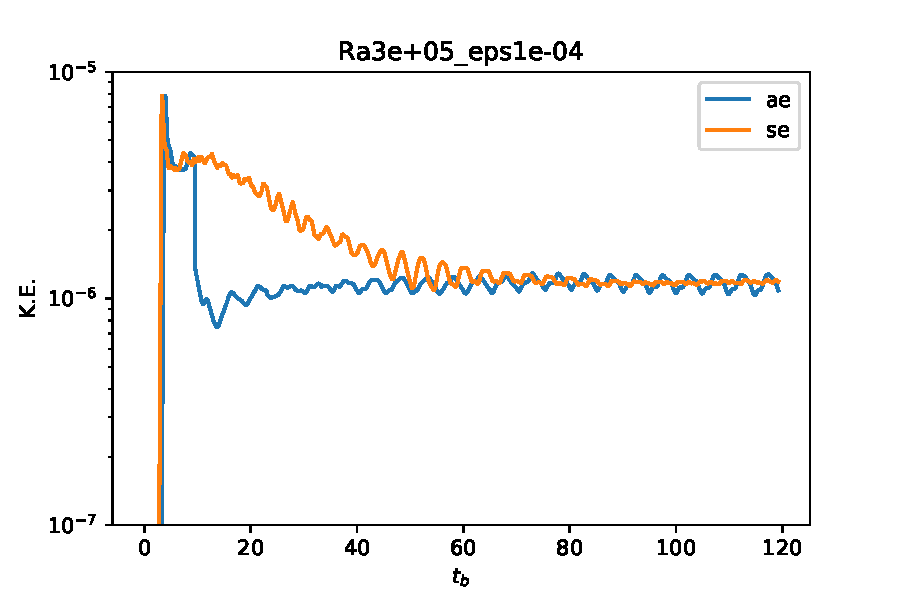
\includegraphics[width=\textwidth]{figs/unpublished/gabo_ae.pdf}
    \caption[Timeseries of kinetic energy in stratified AE vs.~SE.]{
	Kinetic energy trace of a stratified simulation ($\epsilon = 10^{-4}$, supercriticality $\sim 10^4$) comparing AE and SE kinetic energies.
	The AE procedure (described in section \ref{sec:ae}) seems to reach the proper mean value for the converged kinetic energy, but in this instance it put the system into an oscillatory state not achieved by the SE simulation.
    \label{fig:gabo_ae} }
\end{figure}




\subsection{Modifications to the method of Accelerated Evolution}
\label{sec:ae}
For simplicity, we will restrict our study again to FT boundary conditions -- that is, when the flux is fixed at the bottom of the atmosphere, and the temperature is fixed at the top boundary to $T_{\text{top}}$.
We additionally restrict this study to the case in which the thermal conductivity, $\kappa$, is constant.
As described in Sec.~\ref{sec:stability}, we subtract off the adiabatic flux ($\bm{F}_{\text{ad}}$) from the input flux at the bottom boundary ($\bm{F}_{\text{drive}}$) to find the available flux for convection, $\bm{F}_{\text{avail}} = F \hat{z}$, a constant.

In stratified systems, convection carries energy not only through enthalpy fluxes, but also through fluxes of potential energy, kinetic energy, and viscous forces.
All of these new fluxes are driven by convection, and we therefore define the convective flux as in Ch.~\ref{ch:ab17},
\begin{equation}
\bm{F}_{\text{conv}} \equiv \bm{F}_{\text{enth}} + \bm{F}_{\text{KE}} + \bm{F}_{\text{PE}} + \bm{F}_{\text{visc}},
\end{equation}
where $\bm{F}_{\text{enth}} \equiv \rho\bm{u}(c_V T + P/\rho)$ is the enthalpy flux, $\bm{F}_{\text{KE}} \equiv \rho|\bm{u}|^2\bm{u}/2$ is the kinetic energy flux, $\bm{F}_{\text{PE}} \equiv \rho\bm{u}\phi$ (with $\phi \equiv -gz$) is the potential energy flux, and $\bm{F}_{\text{visc}} \equiv -\rho\nu\bm{u}\cdot\lilstressT$ is the viscous flux.
This convective flux combined with the superadiabatic portion of the conductive flux, $\bm{F}_{\text{cond,s}} = -\kappa \grad T - \bm{F}_{\text{ad}}$, will carry $\bm{F}_{\text{avail}}$ through the atmosphere in the evolved state.

As in \citet{anders&all2018}, we find that the fluxes carried through these systems at early times can exceed $F_{\text{avail}}$ as the system leaks out its energy and approaches its relaxed states.
As a result, we define the profile,
\begin{equation}
\xi(z, t) = \frac{F_{\text{avail}}}{F_{\text{conv}} + F_{\text{cond,s}}},
\label{eqn:xi}
\end{equation}
which has a value of unity where the system is carrying the input flux, but whose value is generally less than one at early times while the system is converging.
Here, $\xi$ is a measure of the factor by which the flux through the system must be reduced in order for the system to reach its final, equilibrium state.
In boundary-driven polytropic convection, where $F_{\text{avail}}$ is a uniform, positive value throughout the whole domain, this definition of $\xi$ is fairly robust.
Extensions of the AE method which aim to study stable regions will have to come up with a clever adjustment to $\xi$, but that's beyond the scope of this discussion.

With this definition of $\xi$, we solve a mass-conserving boundary value problem for a modified thermal and hydrostatic equilibrium,
\begin{gather}
\partial_z M_1 = \rho_0(e^{\ln\rho_1} - 1), \\
\kappa\partial_z^2 T_1 = \partial_z(\xi \angles{F_{\text{conv}}}), \\
\partial_z(T_1) + T_1 \partial_z(\ln\rho_0) + T_0\partial_z(\ln\rho_1) = -T_1\partial_z(\ln\rho_1) - \bar{\xi}^{\frac{2}{3}}\angles{\bm{u}\cdot\grad w}.
\end{gather}
with the boundary conditions $M_1 = 0$ at $z = [0, L_z]$, $\partial_z T_1 = 0$ at $z = 0$, and $T_1 = 0$ at $z = L_z$.
Here, the exponent of $\xi^{2/3}$ in the hydrostatic equilibrium equation comes from the assumption that the flux scales like the kinetic energy $F \sim \rho u^3$, so in scaling the flux by $\xi$, we must equivalently scale the velocities by roughly $\xi^{1/3}$.
It's unclear if this is a good assumption.

\subsection{Next steps}
The first obvious next step is to actually see if this procedure works robustly (so far we've only checked it chi-by-eye).
After that, a very important project would be to incorporating a procedure that successfully accounts for stable layers.
It is probable that the knowledge gained in Ch.~\ref{ch:FT20} will be essential in extending AE.
This is to say: thermal relaxation happens in two parts (changes to the energy reservoir and stratification).
AE should likely therefore have two parts (a change to the energy reservoir step based on current flux divergence, and a boundary value problem which solves for the proper stratification under those new energy constraints).


\section{A Freefall Nondimensionalization of the Fully Compressible Equations}
In our standard nondimensionalizations of the fully compressible equations, we nondimensionalize based on the sound speed rather than on the convective velocity (freefall) speed.
In order to compare results with anelastic equations which were nondimensionalized on the freefall timescale, we presented a form of the fully compressible equations in Ch.~\ref{ch:alb19} which were scaled so that one time unit was one freefall time unit. 
However, the version of the fully compressible equations presented in Ch.~\ref{ch:alb19} is essentially nondimensionalized twice, which isn't ideal.
Technically, it is first nondimensionalized on the sound speed and average atmospheric temperature (as in Ch.~\ref{ch:ab17}), and then it is again rescaled based off of the magnitude of thermodynamic perturbations and the freefall velocity.
This works, but it's confusing.
I have faith in the results of the \emph{simulations} from that chapter, which were conducted using a numerical form of the compressible equations similar to the one presented in Ch.~\ref{ch:ab17}, and then rescaled in post-processing.

It would be ideal to have a set of fully compressible equations which are nondimensionalized on the freefall timescale.
This would be useful both for future comparisons to anelastic simulations, but also for numerical stability at low Mach number (where thermodynamic perturbations are O($\epsilon$). O(1) would be better). 
The formulation of the equations that I will derive here aim to understand what the nondimensional fully compressible equations look like when the convective velocities and thermal perturbations are all O(1), regardless of the Mach number.

\subsection{Equation formulation derivation}
We define the fully compressible equations in \citet{anders&brown2017} as:
\begin{gather}
\partial_{\td{t}} \td{\ln \rho_1} + \td{\uvec}\cdot\td{\grad} \td{\ln\rho_0} + \td{\grad}\cdot\td{\uvec} = -\td{\uvec}\cdot\td{\grad}\td{\ln\rho_1} 
\label{eqn:unscaled_continuity}
\\
\begin{split}
\partial_{\td{t}} \td{\uvec} + R(\td{\grad} \td{T_1} + \td{T_1} \td{\grad}\td{\ln\rho_0} + \td{T_0} \td{\grad}\td{\ln\rho_1})
- \td{\nu}\left(\td{\grad}^2 \td{\uvec} + \frac{1}{3}\td{\grad}(\td{\grad}\cdot\td{\uvec}) + \td{\grad}\td{\ln\rho_0}\cdot\td{\lilstressT}\right)
- \td{\grad}\td{\nu}\cdot\td{\lilstressT}
\\= -\td{\uvec}\cdot\td{\grad}\td{\uvec} - R\td{T_1}\td{\grad}\td{\ln\rho_1} + \td{\nu}\td{\grad}\td{\ln\rho_1}\cdot\td{\lilstressT}
\end{split}
\label{eqn:unscaled_momentum}
\\
\begin{split}
\partial_{\td{t}} \td{T_1} + \td{\uvec}\cdot\td{\grad} \td{T_0} + \td{T_0}(\gamma-1)\td{\grad}\cdot\td{\uvec} 
- \frac{c_P}{c_V}\left(\td{\chi}\left\{\td{\grad}^2 \td{T_1} + \td{\grad}\td{\ln\rho_0} \cdot\td{\grad} \td{T_1} + \td{\grad}\td{\ln\rho_1}\cdot\td{\grad} \td{T_0}\right\} 
+ \td{\grad}\td{\chi}\cdot\td{\grad} \td{T_1}\right)
\\= \frac{\td{\chi}c_P}{c_V}\td{\grad}\td{\ln\rho_1}\cdot\td{\grad} \td{T_1} - \td{\uvec}\cdot\td{\grad} \td{T_1} - \td{T_1}(\gamma-1)\td{\grad}\cdot\td{\uvec}
+ \frac{\td{\nu}}{c_V}\td{\lilstressT}\cdot\td{\grad}\cdot\td{\uvec}.
\end{split}
\label{eqn:unscaled_energy}
\end{gather}
Here, the tildes over the terms stand for ``dimensionful" quantities (or quantities that I haven't rescaled yet). 
Those are going to be dropped. 
Only two real assumptions have happened so far: I've assumed hydrostatic equilibrium of the background quantities in the momentum equation, and I've assumed thermal equilibrium of the background quantities in the energy equation.
The rest of this nondimensionalization is predicated around the linearized equation of state,
$$
\frac{\rho_1}{\rho_0} = \frac{P_1}{P_0} - \frac{T_1}{T_0},
$$
and the assumption that for low Mach number flows, each of the quantities in this equation is essentially O($\epsilon$).
We now nondimensionalize all quantities, 
\begin{equation}
\begin{split}
\td{T} =  \bar{T} T, \\
\td{\grad} = L^{-1}\grad,  		\qquad &\partial_{\td{t}} = \tau^{-1}\partial_t, \\
\td{\nu} = \nu\xi(z),				\qquad &\td{\chi} = \chi\xi(z),\\
u_{\ff} = L/\tau, \qquad &%\td{c_V} = R c_V,
\end{split}
\end{equation}
and note that $\ln\rho$ is already dimensionless in its nature.
Here, $\xi(z)$ is the nondimensional shape of the diffusivity profiles.
The nondimensional momentum equation is
\begin{equation}
\begin{split}
\frac{D \bm{u}}{Dt} + \frac{ R \bar{T}}{u_{\text{ff}^2}} \left( \grad T_1 + T_1 \grad \ln\rho_0 + T_0 \grad \ln\rho_1 + T_1 \grad\ln\rho_1\right)
\\
= \frac{\nu \tau}{L^2}\left( \xi\left[\grad^2\uvec + \frac{1}{3}\grad(\DivU) + \grad\ln\rho_0\cdot\lilstressT + \grad\ln\rho_1\cdot\lilstressT\right] + \grad\xi\cdot\lilstressT\right)
\end{split}
\end{equation}
We now make the choice that the nondimensional scale of the temperature perturbations is O($\epsilon$) compared to the background temperature, $\bar{T} = \epsilon T_0$.
Per Ch.~\ref{ch:ab17}, the isothermal Mach number of these flows is roughly $\text{Ma}_{\text{iso}} = \sqrt{\epsilon}$, so the choice that
$$
u_{\text{ff}}= \sqrt{R \bar{T}} \sim \text{Ma}_{\text{iso}} 
$$
means that we're roughly nondimensionalizing on the freefall velocity of the flows.
The continuity and momentum equation under this assumption are then
\begin{gather}
\frac{D \ln\rho_1}{Dt} + (\bm{u}\cdot\ln\rho_0 + \DivU) = 0 \\
\begin{split}
\frac{D \bm{u}}{Dt} + \left( \grad T_1 + T_1 \grad \ln\rho_0 + T_0 \grad \ln\rho_1 + T_1 \grad\ln\rho_1\right)
\\
= \frac{1}{\text{Re}_{\text{ff}}}\left( \xi\left[\grad^2\uvec + \frac{1}{3}\grad(\DivU) + \grad\ln\rho_0\cdot\lilstressT + \grad\ln\rho_1\cdot\lilstressT\right] + \grad\xi\cdot\lilstressT\right)
\end{split}
\end{gather}
where the freefall Reynolds number is
$$
\text{Re}_{\text{ff}} = \frac{u_{\text{ff}} L}{\nu} = \sqrt{\frac{\text{Ra}}{\text{Pr}}}\,\,\,\text{(in the case of convection)}.
$$
The nondimensional temperature equation is
\begin{gather}
\begin{split}
&\frac{D T_1}{Dt} + \left(\uvec\cdot\grad T_0 + (T_0 + T_1)(\gamma-1)\DivU\right)
\\
&= \frac{\chi \tau c_P}{c_V L^2}\left(\xi\left[\grad^2 T_1 + \grad\ln\rho_0\cdot\grad T_1 + \grad\ln\rho_1 \cdot\grad T_0 + \grad\ln\rho_1\cdot\grad T_1\right] + \grad\xi\cdot\grad T_1\right)
 + \frac{\nu}{c_V \bar{T} \tau }\xi\lilstressT\cdot\grad\cdot\uvec.
\end{split}
\end{gather}
The viscous heating term is a bit tricky, but substituting $\bar{T} = u_{\text{ff}}^2/R^2$, we're left with
\begin{equation}
\begin{split}
\frac{D T_1}{Dt} + \left(\uvec\cdot\grad T_0 + (T_0 + T_1)(\gamma-1)\DivU\right)
\\= \frac{c_P}{c_V \text{Pe}_{\text{ff}}}\left(\xi\left[\grad^2 T_1 + \grad\ln\rho_0\cdot\grad T_1 + \grad\ln\rho_1 \cdot\grad T_0 + \grad\ln\rho_1\cdot\grad T_1\right] + \grad\xi\cdot\grad T_1\right)
 + \frac{R^2}{c_V \text{Re}_{\text{ff}} }\xi\lilstressT\cdot\grad\cdot\uvec,
\end{split}
\end{equation}
where
$$
\text{Pe}_{\text{ff}} = \text{Re}_{\text{ff}}\text{Pr}.
$$

Note that it is \emph{crucial} that you consistently nondimensionalize the background temperature profile so that both it--and gravity--are O($\epsilon^{-1}$).
Which is to say that, if you're using a polytrope, rather than $T_0 = 1 + (L_z - z)$, you need to specify
$$
T_0 = \epsilon^{-1}\left(1 + [L_z - z]\right),
$$
and gravity with be $g = (1 + m)/\epsilon$, for $m$ the polytropic index.
Per the polytropic assumption, $\rho = T^m$ still holds, so $\ln\rho_0$ will be shifted by $-\ln(\epsilon)$.

One thing that's nice about this nondimensionalization, in addition to having O(1) flows for numerical stability, is that it's clear to see where the linear wave terms come from.
Any term that has a $T_0$ in it is large, or O($\epsilon^{-1}$) compared to the other terms, so these are the stiff terms in the equations.


\section{Convection with Kramer's Opacity}
\label{sec:kramers_opacity}
All of the experiments presented in this work utilized a constant conductivity.
The Sun, however, has a conductivity which varies by orders of magnitude over the course of its convection zone.
In the optically thick, deep convection zone, the opacity in the Sun can be modeled as a Kramer's Opacity \citep[see e.g.,][]{brandenburg2016}, and the conductivity is a radiative conductively constructed with that opacity choice.
Some recent simulation work by \citet{kapyla&all2017} compared some convection which utilized polytropic-like stratifications with a constant conductivity to simulations with a Kramer's-informed conductivity.
They found some interesting things, including ``Deardorff'' layers, which are layers in the convection zone which are marginally stable but which have a positive convective flux.
They claim that these are only seen with the realistic Kramer's-like opacity.
Internally, as a research group, we have observed extended Deardorff layers even in simpler polytropic atmospheres.
In this project, we had hoped to discover what it is about a Kramer's-like opacity in their simulations that caused them to see such deep Deardorff layers.
In the end, what we learned was that using a Kramer's opacity is difficult in DNS.

\subsection{Single-layer, polytropic atmospheres}
The radiative conductivity in a simulation with a Kramer's opacity \citep{kapyla&all2017} takes the form
$$
\kappa(z) = \kappa_0 \left(\frac{\rho}{\rho_c}\right)^{-(1+a)} \left(\frac{T}{T_c}\right)^{(3-b)}.
$$
The conductivity profile in the solar convection profile is fairly well described by such a formulation with $a = 1$ and $b = -7/2$.
The thermal diffusivity is $\chi = \kappa / (\rho c_P)$. 
If a polytropic atmosphere is assumed ($\rho \propto T^m$), the polytropic index that achieves a constant Kramer's opacity \citep{jones1976} is
$$
m_{kram} = \frac{3 - b}{1 + a}.
$$
Note that if the adiabatic index is $\gamma = 5/3$, then the solar values for $a$ and $b$ produce $m_{kram} = 3.25 > m_{\text{ad}}$ (see Ch.~\ref{ch:ab17}), producing a stable stratification.
However, a choice of $a = 1$ with values of $b = (0, 1]$ get the proper ``flavor'' of this opacity ($\rho^{-2}$, $T^{\text{nonzero integer}}$).
Furthermore, this choice of exponents leads to
\begin{equation}
m_{kram} = 1.5 - b/2 = m_{ad} - b/2.
\end{equation}
So $b$ should behave like $2\epsilon$ from Ch.~\ref{ch:ab17}, driving low or high Mach number flows accordingly.
We had some success simulating these atmospheres (where we set up the initial conditions to have $m = m_{kram}$).

However, when we tried to reproduce some of the results of \cite{kapyla&all2017}, we ran into some roadblocks.
The solar choices of $a = 1$ and $b = -7/2$ in the presence of a perfectly adiabatic atmosphere result in the conductivity dropping by orders of magnitude.
This essentially drives convection which is O(large) and very high Mach number, and also requires impossibly large temperature gradients in the boundary layers to conduct the fluxes.
Past authors used SGS tactics to get around this, but I didn't know how to choose a proper SGS model, nor did I trust that I would be able to consistently interpret and compare simulations with SGS models to those without.

So -- I dropped this project.
However, it is still really unclear how nonlinear conductivities affect convective flows at a fundamental level, and this should be pursued in more detail.

\subsection{A note on implementing a Kramer's Opacity in Dedalus}
A fully nonlinear conductivity is not something that we often deal with in our Dedalus scripts.
However, it's quite easy to implement a Kramer's-informed radiative conductivity (or any nonlinear conductivity) through the following procedure.
If we have a radiative conductivity of the form,
\begin{equation}
\kappa(\ln\rho, T) = \kappa_0 \rho^{-(1 + a)} T^{3 - b}
= \kappa_0 \left(e^{\ln\rho}\right)^{-(1 + a)} T^{3 - b},
\end{equation}
then we can Taylor expand around our thermodynamic variables ($T, \ln\rho$) into constant, linear, and nonlinear components,
\begin{equation}
\kappa(\ln\rho, T) = \kappa(\ln\rho_0, T_0) 
+ \frac{\partial \kappa}{\partial T}\bigg|_{\ln\rho_0, T_0}(T - T_0)
+ \frac{\partial \kappa}{\partial \ln\rho}\bigg|_{\ln\rho_0, T_0}(\ln\rho - \ln\rho_0)
+ \kappa_{\text{NL}}.
\end{equation}
To evaluate that, we need a couple of derivatives:
\begin{equation}
\begin{split}
&\frac{\partial \kappa}{\partial T}\bigg|_{\rho_0, T_0} = 
\kappa_0(3-b)\rho_0^{-(1+a)}T_0^{2-b} = (3-b)\frac{\kappa(\ln\rho_0, T_0)}{T_0} \\
&\frac{\partial \kappa}{\partial \ln\rho}\bigg|_{\rho_0, T_0} =
\rho\frac{\partial \kappa}{\partial \rho}\bigg|_{\rho_0, T_0} =
-(1+a)\kappa_0 \rho_0^{-(1+a)} T_0^{3-b} = -(1+a)\kappa(\ln\rho_0, T_0),
\end{split}
\end{equation}
and after quick substitutions,
\begin{equation}
\kappa(\rho, T) = \kappa(\rho_0, T_0)\left( 1 +
(3 - b)\frac{T_1}{T_0} - (1 + a) \ln\rho_1 \right)
+ \kappa_{\text{NL}}
\end{equation}
At this point, I will define the constant, linear, and nonlinear parts of $\kappa$,
\begin{equation}
\begin{split}
&\kappa_\text{C} \equiv \kappa(\rho_0, T_0) \\
&\kappa_\text{L} \equiv \kappa_C\left(
(3 - b)\frac{T_1}{T_0} - (1 + a) \ln\rho_1 \right) \\
&\kappa_{\text{NL}} \equiv \kappa - \kappa_\text{C} - \kappa_{\text{L}}.
\end{split}
\end{equation}
Note that the trick here is that we peel away the constant (trivial) and linear (easy) portions of the conductivity from the full, hard opacity.
In general, at least at low Mach number, $\kappa_{NL}$ is likely quite small.

The LHS of the energy equation has a term
\begin{equation}
\text{DivFcond} = \Div{-\kappa\grad T} 
= -(\kappa\grad^2 T + \grad \kappa\cdot\grad T),
\end{equation}
which can be simply broken up into linear (L) and nonlinear (NL) components,
\begin{equation}
\begin{split}
&\text{DivFcond\_L} = -\left(\kappa_\text{L}\grad^2 T_0 
+ \kappa_\text{C} \grad^2 T_1 
+ \grad T_0 \cdot \grad \kappa_\text{L}
+ \grad T_1 \cdot \grad \kappa_\text{C}\right) \\
&\text{DivFcond\_NL} = -\left(
(\kappa - \kappa_\text{L})\grad^2 T_0
+ (\kappa - \kappa_\text{C})\grad^2 T_1
+ \grad T_0 \cdot \grad(\kappa - \kappa_\text{L}) 
+ \grad T_1 \cdot \grad(\kappa - \kappa_\text{C}) \right),
\end{split}
\end{equation}
where the background profile has here been assumed to be in thermal equilibrium.


\section{Turbulent Thermals}
\label{sec:turb_thermals}
\begin{figure*}[p!]
    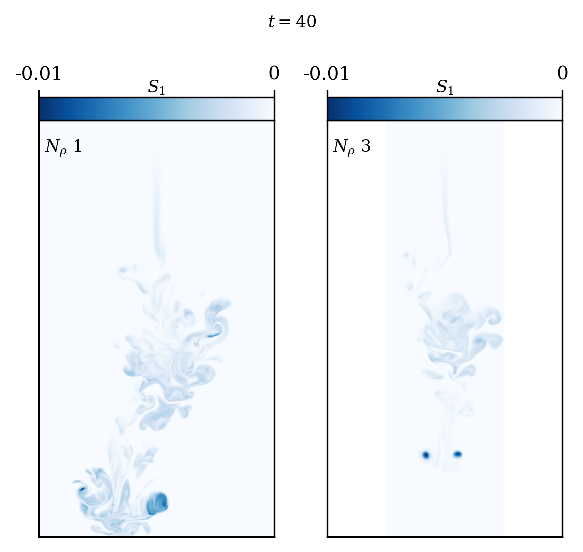
\includegraphics[width=\textwidth]{figs/unpublished/turbulent_thermals.pdf}
    \caption[Evolved turbulent thermals]{
	Horizontal slices through Cartesian domains containing evolved turbulent thermals.
	In both cases, the initial freefall Reynolds number of the thermals is $4\cdot10^3$.
	On the left is an evolved thermal in a 1-density-scale-height atmosphere.
	On the right is an evolved thermal in a 3-density-scale-height atmosphere.
	There are two observations that can be made from this figure that are strange.
	First, the vortex ring on the right looks quite laminar, whereas the one on the left looks quite turbulent.
	Second, unlike in the results of Ch.~\ref{ch:alb19}, the thermal in the highly stratified atmosphere is falling \emph{slower} than the one on the right.
    \label{fig:turbulent_thermals} }
\end{figure*}


The next logical step in the study presented in Ch.~\ref{ch:alb19} is a study of turbulent thermals.
I have performed some initial simulations of anelastic, 3D thermals at Re = $4 \cdot 10^3$, but the initial results from these simulations are rather perplexing.
See Fig.~\ref{fig:turbulent_thermals}.

While simulations of thermals are not computationally expensive in \emph{time} (they are short), they are expensive in terms of \emph{memory}.
Even the laminar simulations presented in Ch.~\ref{ch:alb19} took many coefficients to resolve, and were nearly at the limits of our computational abilities on a system like NASA Pleiades.
Increasing the turbulence (the Reynolds number) by an order of magnitude is therefore quite difficult.
In order to get around this problem, we changed the formulation of our diffusivities.
Rather than holding the \emph{dynamic} diffusivities constant (as we did in Ch.~\ref{ch:alb19}), we here held the diffusivities (in units of cm$^2$/s) constant.
This means that the dynamic viscosities grow proportionally to density.
Importantly, in compressible or anelastic domains, this means that the viscous heating term (in the equation for total entropy or for total energy) grows with density.
This choice seems to eat away at the buoyant signature of our dense thermals by heating them as they fall, and this in turn reduces the thermal acceleration.
This messes up our theory, because we assumed the buoyant signature was constant in time.

The theory of thermals that we derived in Ch.~\ref{ch:alb19} revolved around the \emph{momentum} and the \emph{entropy} (which is density-weighted, unlike the specific entropy).
The form of the diffusivities that appear in the equations for those quantities are the \emph{dynamic} diffusivities, which in these initial turbulent simulations grow with depth.
Moreover, they grow more with depth in a highly stratified atmosphere than they do in an atmosphere which is not highly stratified.
These initial results suggest that if one wants to study dynamics which are equally turbulent throughout the full depth of an atmosphere, the ``proper'' choice of diffusivities is to hold the dynamic diffusivities constant, meaning that the diffusivities shrink with depth like $\rho$.

Regardless, these initial struggles and the high computational expense of turbulent thermals have currently caused this project to stall out.
Furthermore, from some conversations with Mark Rast, there is some reason to perhaps be concerned about simulating cylindrical structures in Cartesian domains \citep[see e.g., Fig.~9 of][]{clyne&all2007}, as the shape of the domain can lead to non-axisymmetric unrealistic perturbations.
The striking similarity reported between 2D (cylindrical) and 3D (Cartesian) domains in Ch.~\ref{ch:alb19} gives optimism that those calculations should be trusted, but it would likely be ideal to conduct future experiments in cylindrical domains if possible.
Beyond this more subtle numerical problem, it is unclear if our initial conditions (thermals) are the ``right'' experiment (e.g., are thermals or plumes the basic convective element?).
A review of this debate in the context of Earth's atmosphere is laid out in detail by \citet{yano2014}.


